% !TEX root = pfc.tex

Segundo \cite{linda:2001:book}, visão computacional é um campo da Ciência da Computação que inclui métodos para a aquisição, processamento e análise de imagens. \cite{morris:2004:book} define processamento de imagem e visão computacional separadamente. Para \citeauthor{morris:2004:book}, processamento de imagem é a manipulação de uma imagem digital, gerando como resultado uma nova representação da mesma imagem, ao passo que visão computacional é a extração de informações numéricas ou simbólicas de imagens. Em linhas gerais, visão computacional é a tecnologia que transforma imagens do mundo real em uma representação que computadores são capazes de interpretar e processar e, com isso, produzir informações úteis para aplicações de Engenharia. Contempla uma base teórica e tecnológica para a construção de sistemas artificiais que obtém informações de imagens ou quaisquer dados multidimensionais. Mas como os computadores podem entender o mundo visual dos humanos? Quais vantagens e quais tipos de aplicações podem existir a partir desse conceito?

Segundo \cite{szeliski:2010:book}, o ser humano é perfeitamente capaz de perceber a estrutura tridimensional do mundo ao seu redor. Ao visualizar a Figura \ref{fig:flower}, percebe-se que a visão humana interpreta variações de transparência e sombra, além de diferenciar o objeto do \textit{backgroud}\footnote{Segundo plano ou plano de fundo} com facilidade. Isso acontece porque o cérebro humano divide o sinal de visão em muitos canais, gerando um fluxo de diferentes tipos de informação. Ele é capaz de identificar as partes importantes de uma imagem a serem examinadas e ao mesmo tempo suprimir a atenção para regiões menos importantes \citep{szeliski:2010:book}. Além disso, o cérebro possui um sistema de realimentação poderoso que implementa um controle em malha fechada, composto por sensores (visão, audição, olfato, tato e paladar) e atuadores (íris para controlar a entrada de luminosidade nos olhos) \citep{opencv:2008:book}.

\begin{figure}[ht]
  \begin{center}
    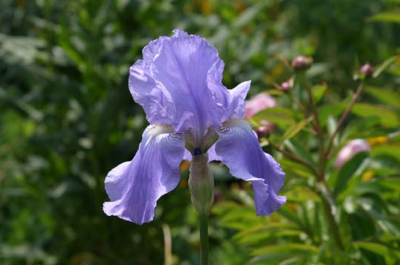
\includegraphics{imgs/flower.png}
  \end{center}
  \caption{O ser humano é capaz de determinar a forma e a transparência de cada pétala de uma flor \citep{szeliski:2010:book}.}
  \label{fig:flower}
\end{figure}

Diante da facilidade com que o ser humano enxerga o mundo ao seu redor é intuitivo pensar que o processamento de imagens por visão computacional é simples. Mas isso não é verdade. Em um sistema de visão, o computador recebe, na maioria das vezes, apenas uma matriz de números inteiros, em que cada posição é denominada pixel, como mostrado na Figura \ref{fig:opencv_car}. Todos aqueles padrões de interpretação de informação presentes no cérebro não existem aqui. Além disso, deve-se considerar os ruídos existentes num sistema de visão, que diminuem ainda mais a quantidade de informação dos dados. Esse tipo de problema pode ser causado devido a variações no ambiente (luminosidade, clima, reflexos, movimentações), imperfeições na captura de imagem (lente, configuração mecânica), ruídos elétricos no sensor óptico da câmera e compressão das imagens após a captura \citep{opencv:2008:book}.

\begin{figure}[ht]
  \begin{center}
    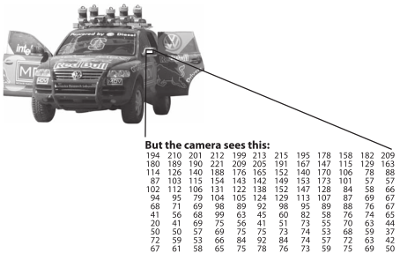
\includegraphics{imgs/opencv_car.png}
  \end{center}
  \caption{Para um computador, o retrovisor de um carro é apenas uma matriz composta por pixeis \citep{opencv:2008:book}.}
  \label{fig:opencv_car}
\end{figure}

Mesmo com todos esses desafios, por incrível que pareça, é possível desenvolver sistemas baseados em visão computacional bastante robustos e com alto grau de confiabilidade. Isso começa a se tornar possível quando as imagens capturadas estão inseridas no contexto de uma determinada aplicação. Por exemplo: se um sistema de visão computacional tem por objetivo rastrear carros, não faz nenhum sentindo buscar os veículos em áreas que não sejam as ruas, avenidas e rodovias. Caso um objeto seja encontrado em uma área verde ou no azul do céu, a probabilidade de que esse objeto seja um carro é muito baixa. É uma análise óbvia mas de suma importância no processamento de imagens.

O uso de métodos estatísticos em visão computacional também são primordiais, convergindo para o problema de ruído discutido anteriormente. Considerar a média dos pixeis no tempo é uma abordagem estatística, que pode vir a ser uma solução para problemas que envolvem imagens ruidosas. Outra técnica bastante comum é a construção de modelos das câmeras, capazes de caracterizá-las matematicamente através de seus parâmetros intrínsecos e extrínsecos. Os parâmetros internos da câmera como distância focal, distorções de lente e tamanho do pixel correspondem aos parâmetros intrínsecos. Os parâmetros extrínsecos estão relacionados à orientação e posição da câmera em relação a um sistema de referência no mundo. Com esses parâmetros fica simples corrigir imperfeições nas imagens, que podem ocorrer devido a lente ou alguma configuração mecânica \citep{opencv:2008:book}.

Essas e mais uma série de técnicas, descritas nas seções seguintes, são objetos de estudo no campo de visão computacional. Elas em conjunto são combinadas e organizadas de maneira a transformar quaisquer dados multidimensionais em informações de alto nível, como por exemplo ausência e presença de um componente, dimensão e cor de objetos. Como regra geral: quanto mais restrito é o escopo de uma aplicação de visão computacional, mais o problema pode ser simplificado e mais confiável será a solução final \citep{opencv:2008:book}.

A seguir é realizado uma breve revisão bibliográfica sobre conceitos, técnicas e métodos de processamento de imagens digitais aplicados ao campo da visão computacional.

\section{Imagem digital} % (fold)
\label{sec:imagem_digital}

De acordo com \cite{woods:2000:book}, uma imagem pode ser definida como uma função bidimensional de intensidade de luz $f(x,y)$, em que $x$ e $y$ são cordenadas espaciais de um plano, e a amplitude de $f$ é proporcional ao brilho (ou níveis de cinza) da imagem naquele ponto. A Figura \ref{fig:imagem_digital} ilustra a convenção dos eixos adotada nesse e na maioria dos trabalhos da área.

\begin{figure}[ht]
  \begin{center}
    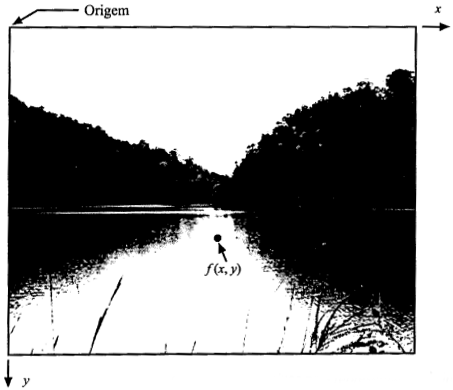
\includegraphics[scale=0.7]{imgs/imagem_digital.png}
  \end{center}
  \caption{Convenção dos eixos para representação de imagens digitais \citep{woods:2000:book}.}
  \label{fig:imagem_digital}
\end{figure}

Uma imagem digital é a discretização de uma imagem $f(x,y)$, tanto em coordenadas espaciais quanto em intensidade de brilho. A OpenCV 2 \citep{opencv_library}, uma biblioteca de visão computacional descrita na Seção \ref{sec:biblioteca_opencv}, considera a imagem digital como sendo uma matriz cujos índices de linhas e colunas determinam um ponto na imagem, e o valor correspondente do elemento da matriz identifica o nível de cinza naquele ponto. Os elementos dessa matriz digital são chamados de pixels, embora existam outros nomes como elementos da imagem, elementos da figura ou pels \citep{woods:2000:book}.

% section imagem_digital (end)

\section{Modelo RGB de cores} % (fold)
\label{sec:modelo_rgb_de_cores}

Segundo \cite{woods:2000:book}, é comprovado que o olho humano possui entre 6 e 7 milhões de cones\footnote{Células fotorreceptoras, localizadas na retina do olho, que são responsáveis pela visão das cores.}, que podem ser dividos em três principais categorias de sensoriamento, aproximadamente correspondentes às cores vermelho, verde e azul. Desse total de cones existentes, cerca de 65\% são sensíveis à luz vermelha, 33\% são sensíveis à luz verde e apenas 2\% deles são sensíveis à luz azul, sendo os cones azuis os que possuem maior grau de sensibilidade à luz. Dessa forma, as cores são vistas pelo olho humano como combinações das chamadas cores primárias: vermelho (R, \textit{red}), verde (G, \textit{green}) e azul (B, \textit{blue}), fato que inspirou estudos do modelo RGB de cores.

O modelo RGB é um sistema de coordenadas cartesianas, onde o sub-espaço das cores de interesse é representado pelo cubo da Figura \ref{fig:cubo_rgb}. Nesse modelo, as cores são pontos sobre ou dentro do cubo, definidas por vetores que estendem-se a partir da origem. A escala de cinza é definida pela diagonal principal desse cubo e assume valores do preto, localizado na origem, ao branco, no vértice mais distante \citep{woods:2000:book}.

Em representações computacionais desse modelo os componentes R, G e B, denominados canais de cor, assumem valores inteiros de uma escala que vai de 0 a 255, possibilitando que cada valor seja armazenado por 1 \textit{byte}\footnote{Unidade de medida de armazenamento de memória em computação. Cada \textit{byte} contém 8 \textit{bits}, suficiente para endereçar $2^8$ números binários.}. Dessa forma, é possível gerar exatamente 16.777.216 (ou $256^3$) combinações de cores diferentes. A Figura \ref{fig:colorcube} ilustra o gradiente formado na superfície do cubo RGB quando os pontos assumem valores inteiros num intervalo de 0 a 255.

\begin{figure}[ht]
  \begin{center}
    \begin{subfigure}[b]{.49\textwidth}
      \begin{center}
        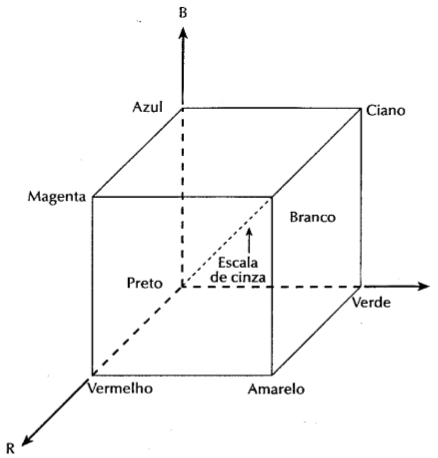
\includegraphics[width=.85\linewidth]{imgs/cubo_rgb.png}
      \end{center}
      \caption{}
      \label{fig:cubo_rgb}
    \end{subfigure}
    \begin{subfigure}[b]{.49\textwidth}
      \begin{center}
        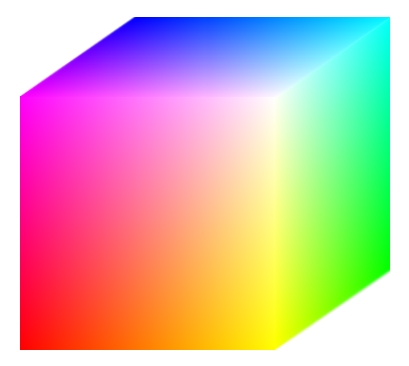
\includegraphics[width=.9\linewidth]{imgs/colorcube.png}
      \end{center}
      \caption{}
      \label{fig:colorcube}
    \end{subfigure}
  \end{center}
  \caption{(a) Cubo de cores RGB. Os pontos ao longo da diagonal principal têm valores da escala de cinza que vão do preto $(0,0,0)$ ao branco $(255,255,255)$ \citep{woods:2000:book}; (b) Representação em cores do cubo RGB \citep{theo:2003:online}.}
  \label{fig:cubos}
\end{figure}

% section modelo_rgb_de_cores (end)

\section{Escala de cinza} % (fold)
\label{sec:escala_de_cinza}

A escala de cinza é muito utilizada em processamento de imagens digitais por ter menor custo computacional. Em imagens RGB são necessários 3 \textit{bytes} (um por canal) para definir a cor de um pixel, enquanto que em imagens \textit{grayscale}\footnote{Escala de cinza.} a representação da cor de um pixel utiliza apenas 1 \textit{byte}, um terço de uma imagem RGB. De acordo com \cite{woods:2000:book}, sistemas de visão computacional em que a cor não é um requisito, é essencial converter as imagens RGB para \textit{grayscale} antes de qualquer operação, como mostrado na Figura \ref{fig:flowers}, diminuindo assim o peso do processamento digital.

Para obter uma imagem \textit{grayscale} a partir de uma imagem RGB deve-se considerar a média da intensidade de cada canal. Essa conversão é dada pela equação 

\begin{gather}
\label{eq:conversao_cinza}
  C_{xy}=(k_{R}\times R_{xy})+(k_{G}\times G_{xy})+(k_{B}\times B_{xy})\text{,}\\
  \nonumber k_{R}, k_{G}, k_{B} > 0 \text{ e }  k_{R}+k_{G}+k_{B}=1\text{,}
\end{gather}

\noindent onde $x$ e $y$ representam a posição do pixel no plano espacial da imagem segundo a convenção de eixos descrita na Seção \ref{sec:imagem_digital}; $C_{xy}$ a intensidade resultante dos pixels na escala de cinza; $R_{xy}$, $G_{xy}$ e $B_{xy}$ a intensidade dos pixels dos canais vermelho, verde e azul, respectivamente; e $k_{R}$, $k_{G}$ e $k_{B}$ constantes relacionadas à sensibilidade de incidência de luz de cada canal de cor \citep{sjohnson:2006:book}. A OpenCV 2 \citep{opencv_library} utiliza os seguintes valores para as constantes: $k_{R}=0.299$, $k_{G}=0.587$ e $k_{B}=0.114$ \citep{opencv_doc:2013:online}.

\begin{figure}[ht]
  \begin{center}
    \begin{subfigure}[b]{.49\textwidth}
      \begin{center}
        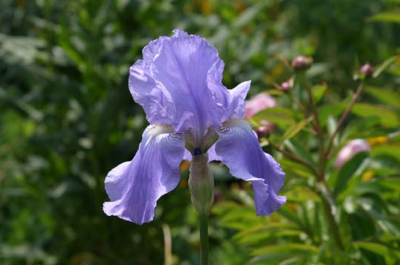
\includegraphics[width=.9\linewidth]{imgs/flower.png}
      \end{center}
      \caption{}
      \label{fig:flower_rgb}
    \end{subfigure}
    \begin{subfigure}[b]{.49\textwidth}
      \begin{center}
        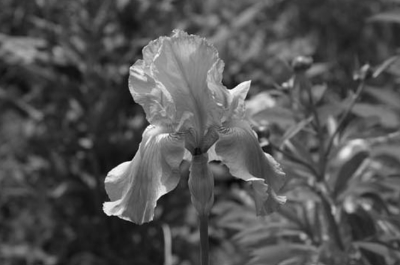
\includegraphics[width=.9\linewidth]{imgs/flower_gray.png}
      \end{center}
      \caption{}
      \label{fig:flower_gray}
    \end{subfigure}
  \end{center}
  \caption{Exemplo de conversão para \textit{grayscale}. (a) Imagem original RGB; (b) Imagem em escala de cinza.}
  \label{fig:flowers}
\end{figure}

% section escala_de_cinza (end)

\section{Histograma} % (fold)
\label{sec:histograma}

Histograma é um gráfico matemático que representa a distribuição de frequências de uma massa de medições \citep{lancaster1973introduction}. Normalmente é representado por retângulos na vertical, onde cada retângulo corresponde a um intervalo e sua altura é proporcional ao número de ocorrências naquele intervalo.

Em visão computacional, os histogramas são utilizados para representar o número de ocorrências de cada cor em uma imagem, como ilustra a Figura \ref{fig:histograma}. Normalmente, é gerado um histograma para cada canal de cor em imagens coloridas, já que pode existir uma infinidade de cores possíveis. O histograma pode proporcionar um melhor entendimento da imagem pois facilita a visualização de parâmetros como contraste e luminosidade.

\begin{figure}[ht]
  \begin{center}
    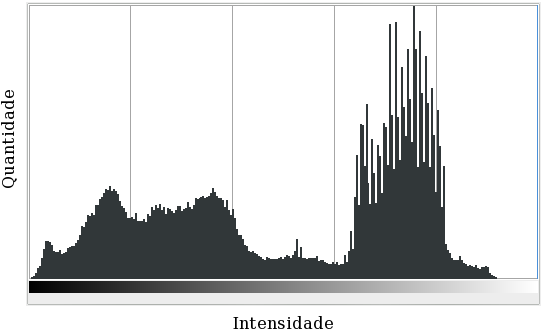
\includegraphics[scale=.55]{imgs/histograma.png}
  \end{center}
  \caption{Histograma de uma imagem \textit{grayscale} gerado pelo \textit{software} \cite{gimp:2013:online}.}
  \label{fig:histograma}
\end{figure}

% section histograma (end)

\section{Filtragem linear} % (fold)
\label{sec:filtragem_linear}

A filtragem linear é um tipo de operação local que considera pixels vizinhos de um determinado ponto para calcular seu novo valor, como ilustrado na Figura \ref{fig:convolucao}. Operadores locais, ou operadores de vizinhança\footnote{Tradução livre de \textit{neighborhood operators}} como são mais conhecidos, são muito utilizados no processamento digital de imagens e podem ser usados como filtros espaciais lineares para gerar efeitos de borramento, acentuação de bordas, remoção de ruídos, entre outros.

\begin{figure}[ht]
  \begin{center}
    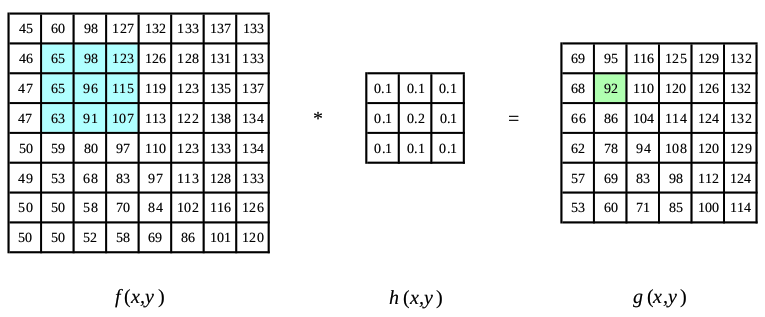
\includegraphics[scale=.58]{imgs/img_convolucao.png}
  \end{center}
  \caption{Filtragem linear por convolução: a imagem da esquerda convolução com o filtro no centro produz a imagem da direita. Os pixels em destaque de $f(x,y)$ indicam a vizinhança usada para gerar o pixel em destaque na saída $g(x,y)$ \citep{szeliski:2010:book}.}
  \label{fig:convolucao}
\end{figure}

De acordo com \cite{szeliski:2010:book}, filtros lineares são os operadores de vizinhança mais usados, em que o valor de saída $g(i,j)$ é determinado por uma soma ponderada de valores de pixels de entrada $f(i+k,j+l)$ (Figura \ref{fig:convolucao}),

\begin{equation}
  \label{eq:correlacao}
  g(i,j)=\sum_{k,l}f(i+k,j+l)h(k,l)\text{.}
\end{equation}

\noindent A ponderação é dada pelo \textit{kernel} ou máscara $h(k,l)$, que contém os coeficientes do filtro, responsáveis pelas características de suavização, borramento ou remoção de ruídos inerentes a cada tipo de filtragem. A Equação \eqref{eq:correlacao} é um estimador do conhecido operador de correlação, que na forma compacta pode ser escrito como

\begin{equation}
  \label{eq:correlacao_compac}
  g=f\otimes h\text{.}
\end{equation}

Uma variação muito comum de filtro, como o apresentado em \eqref{eq:correlacao}, é dada por:

\begin{equation}
  \label{eq:convolucao}
  g(i,j)=\sum_{k,l}f(i-k,j-l)h(k,l)=\sum_{k,l}f(k,l)h(i-k,j-l)\text{,}
\end{equation}

\noindent onde o sinal dos deslocamentos em $f$ foram invertidos. Essa é um estimador da chamada operação de convolução,

\begin{equation}
  \label{eq:convolucao_compac}
  g=f*h\text{.}
\end{equation}

% As operações de correlação e convolução são equivalentes, a não ser pela fase de 180° que gera uma rotação no processo de filtragem por correlação. Elas são a base matemática para implementação de qualquer tipo de filtro linear, como por exemplo, \textbf{gaussiano}.

\begin{figure}[ht]
  \begin{center}
    \begin{subfigure}[b]{.49\textwidth}
      \begin{center}
        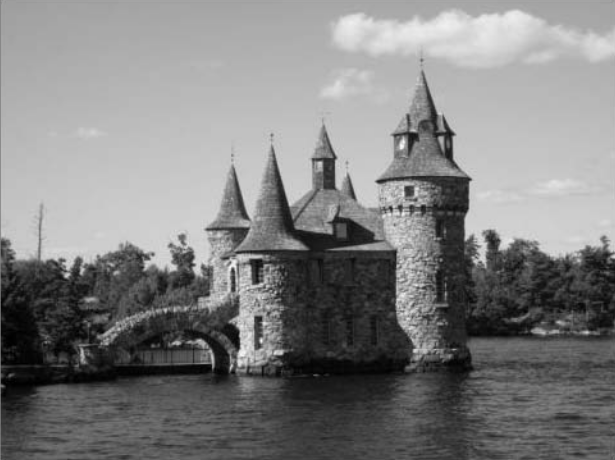
\includegraphics[width=.9\linewidth]{imgs/castelo_original.png}
      \end{center}
      \caption{}
      \label{fig:castelo_orig}
    \end{subfigure}
    \begin{subfigure}[b]{.49\textwidth}
      \begin{center}
        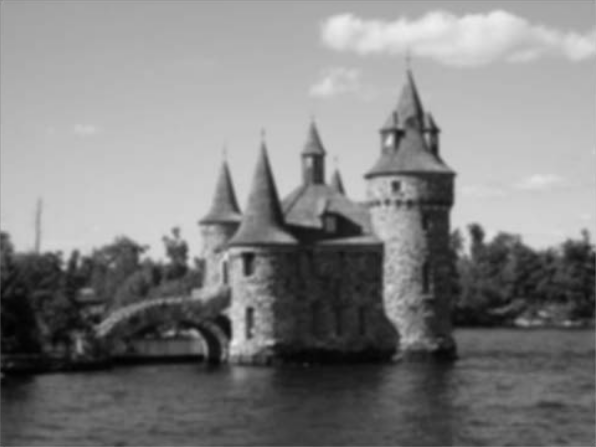
\includegraphics[width=.9\linewidth]{imgs/castelo_gaussiano.png}
      \end{center}
      \caption{}
      \label{fig:castelo_gauss}
    \end{subfigure}
  \end{center}
  \caption{Percebe-se o comportamento passa-baixa do filtro atenuando componentes de alta frequência na imagem (bordas). (a) Imagem original; (b) Aplicação de filtragem linear gaussiana \citep{opencv2:2011:book}.}
  \label{fig:filtro_gaussiano}
\end{figure}

Segundo \cite{opencv_doc:2013:online}, o filtro gaussiano é talvez o mais útil entre todos. É largamente utilizado no processamento de imagens digitais para remoção de ruídos e redução de detalhes, como ilustrado na Figura \ref{fig:filtro_gaussiano}, onde pode-se verificar um suave borramento e a diminuição de detalhes nas bordas, características típicas de um filtro passa-baixa. A filtragem é feita através da convolução de cada pixel da imagem de entrada por um \textit{kernel} cujos valores obedecem uma distribuição gaussiana bidimensional, representada por

\begin{equation}
  \label{eq:gaussian_blur}
  h(k,l)=Ae^{\dfrac{-(k-\mu_{k})^{2}}{2\sigma_{k}^{2}}+\dfrac{-(l-\mu_{l})^{2}}{2\sigma_{l}^{2}}}\text{,}
\end{equation}

\noindent onde $\mu$ é a média e $\sigma$ o desvio padrão. Nessa configuração, os pixels mais próximos de $\mu$ têm maior peso no resultado, portanto são mais significativos para o cálculo da intensidade de cada ponto. O peso dos pixels vizinhos decai com a distância e é influenciado também pelo desvio padrão $\sigma$.

% section filtragem_linear (end)

\section{Limiarização} % (fold)
\label{sec:limiariza_o}

Segundo \cite{opencv:2008:book}, a operação de limiarização, também conhecida por \textit{thresholding}, é o método de segmentação em imagens digitais mais simples que existe. Essa técnica pode ser aplicada para separar regiões correspondentes a objetos que se deseja analisar, como iustrado na Figura \ref{fig:threshold_maca}.

\begin{figure}[ht]
  \begin{center}
    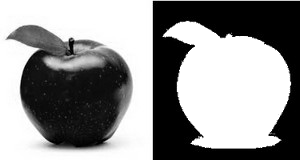
\includegraphics{imgs/threshold_maca.png}
  \end{center}
  \caption{Segmentação de uma maçã utilizando limiarização binária \citep{opencv_doc:2013:online}.}
  \label{fig:threshold_maca}
\end{figure}

A separação se dá pela diferença de intensidade entre os pixels do objeto e os pixels pertencentes ao plano de fundo. Para diferenciar os pixels de interesse é feito uma comparação do nível de cinza de cada pixel com um limiar (ou valor de \textit{threshold}), que pode ser uma constante determinada de acordo com as necessidades do problema ou uma variável em algoritmos de limiarização adaptativos. Uma vez que os pixels de interesse foram segmentados, basta determinar um valor comum para identificá-los, sendo mais comum o branco 255 (Figura \ref{fig:threshold_maca}).

No caso geral, a operação de limiarização binária é dada por

\begin{equation}
  dst(x,y)=\begin{cases}
    maxVal & \text{se $src(x,y) > thresh$}\\
    0 & \text{caso contrário.}
  \end{cases}
\end{equation}

\noindent Portanto, se a intensidade do pixel $src(x,y)$ é maior que o limiar $thresh$, então a nova intensidade do pixel $dst(x,y)$ será $maxVal$; caso contrário, é atribuído a $dst(x,y)$ o valor 0 (preto) \citep{opencv:2008:book}.

% section limiariza_o (end)

% \section{Subtração de fundo} % (fold)
% \label{sec:subtra_o_de_background}

% % section subtra_o_de_background (end)

% \section{Operações morfológicas} % (fold)
% \label{sec:opera_es_morfol_gicas}

% \subsection{Erosão} % (fold)
% \label{sub:eros_o}

% \subsection{Dilatação} % (fold)
% \label{sub:dilata_o}

% \subsection{Abertura e fechamento} % (fold)
% \label{sub:abertura_e_fechamento}

% % subsection abertura_e_fechamento (end)

% % subsection dilata_o (end)

% % subsection eros_o (end)

% % section opera_es_morfol_gicas (end)

% \section{Detecção de características relevantes} % (fold)
% \label{sec:detec_o_de_caracter_sticas_relevantes}

% % section detec_o_de_caracter_sticas_relevantes (end)

\section{Biblioteca OpenCV} % (fold)
\label{sec:biblioteca_opencv}

OpenCV (\textit{Open Source Computer Vision}) \citep{opencv_library} é uma biblioteca de visão computacional \textit{open source} disponível em: \url{http://sourceforge.net/projects/opencvlibrary/}. O código é escrito em C e C++ e pode ser compilado e executado em ambientes Linux, Windows e Mac OS X. Existem também interfaces em Python, Ruby, Matlab e outras linguagens. Contém mais de 500 algoritmos otimizados para processamento de imagens e vídeos, cobrindo diversas áreas da visão computacional, como: inspeção industrial, imagens médicas, segurança, interface com o usuário, calibração de câmera, visão estéreo, robótica e \textit{machine learning} \citep{opencv:2008:book}.

Segundo \cite{opencv2:2011:book}, desde o lançamento da OpenCV em 1999, ela vem sendo largamente adotada como a principal ferramenta de desenvolvimento pela comunidade de pesquisadores e programadores em visão computacional. A biblioteca foi originalmente desenvolvida pela Intel \citep{intel:2013:online}, por um time liderado por Gary Bradski e com o propósito de avançar em pesquisas na área de visão. Depois de uma série de versões \textit{Beta}, a versão 1.0 foi lançada em 2006. O segundo maior lançamento aconteceu em 2009 com a OpenCV 2, propondo importantes modificações em sua estrutura e especialmente a nova interface C++. Atualmente a OpenCV encontra-se na versão 2.4.

\cite{opencv:2008:book} afirmam que a licença \textit{open source} da OpenCV permite que aplicações comerciais possam ser construídas utilizando parte ou toda a biblioteca, sem a necessidade de que o código da aplicação seja aberto. Devido a essa política liberal de uso, gigantes como IBM, Microsoft, Intel, SONY, Siemens, Google, além dos centros de pesquisa Stanford, MIT, CMU, Cambridge e INRIA, utilizam a biblioteca em seus projetos e pesquisas. A OpenCV foi peça chave no sistema de visão de um robô desenvolvido em Stanford, conhecido como Stanley, que ganhou a corrida de carros autônomos \textit{\$2M DARPA Grand Challenge}.
%\citep{thrun:2006:article}. Um relato desse caso é feito na Subseção \ref{sub:dire_o_aut_noma_de_ve_culo_inteligente}.

%TODO: colocar tabela com as funçoes c++

% section biblioteca_opencv (end)

\section{Aplicações existentes} % (fold)
\label{sec:aplica_es_existentes}

\cite{ivision:2013:online} possui diversas aplicações concebidas utilizando os conhecimentos de visão computacional. O fato dessa tecnologia ser não intrusiva, ou seja, não altera em nada o meio em que está sendo utilizada, torna os sistemas de visão realizáveis em grande parte dos processos industriais, urbanos e ambientais.

As aplicações em análise dimensional se caracterizam por efetuarem medidas em objetos, sendo elas lineares e/ou angulares. A análise dimensional por imagem é vantajosa pois possibilita que as medidas sejam feitas à distância, quando não é possível ou desejável o contato direto com o objeto. Câmeras de alta resolução se aplicam nesses projetos, garantindo medições precisas e com repetibilidade. Muito comum na siderurgia, esse tipo de aplicação possibilita a medição em objetos que se encontram em altas temperaturas. As câmeras infravermelho têm sido utilizadas nesse tipo de aplicação.

O uso de reconhecimento de padrões permite a identificação de características de um produto comparando-o com um modelo predeterminado. Essas características a serem inspecionadas são escolhidas para identificar e diferenciar um tipo de modelo de outro. Assim é possível dizer se um objeto está conforme um padrão ou não.

Inspeção de nível é bastante comum na indústria de bebidas e na indústria farmacêutica para inspeção de enchimento de ampolas, vidros de medicamentos ou qualquer recipiente translúcido que contenha líquido.

A inspeção por análise de cores possibilita a criação de soluções para separar produtos por cor ou verificar se a tonalidade está igual a uma amostra. Tem a vantagem de ser um método determinístico em relação a uma inspeção de cores realizada por seres humanos, onde pode existir subjetividade. No entanto, variações de luminosidade podem dificultar a realização desse tipo de inspeção.

Existem também aplicações de rastreabilidade que envolvem leituras de códigos de barras ou de códigos bidimensionais como \textit{Data Matrix}\footnote{Código de barras matricial bi-dimensional que consiste em células brancas ou pretas arranjadas em forma de quadrado ou retângulo. Caracteriza-se pelas bordas em formato de L. Armazena no máximo 2335 caracteres alfanuméricos.} e o \textit{QR Code}\footnote{\textit{Quick Response Code} é um código de barras bi-dimensional criado pela empresa japonesa Denso-Wave em 1994. Pode armazenar até 7089 caracteres, dependendo do tipo de dado. Possui redundância em sua codificação, possibilitando correção e recuperação de informação.}. Permitem identificar e rastrear os produtos, bem como armazenar grandes quantidades de dado. São sistemas frequentemente utilizados na indústria automobilística mas são aplicáveis em qualquer projeto que necessite de controle de produção.

As aplicações para contagem, seleção e classificação podem instrumentar diversas indústrias, como por exemplo a indústria farmacêutica para contagem de medicamentos. Também é comum na produção de componentes eletrônicos para verificação de pinos e conectores. Na engenharia de transporte podem contribuir na análise do tráfego realizando contagem volumétrica de veículos e pessoas, classificação e caracterização de veículos quanto ao tamanho e forma e leitura de placas utilizando técnicas de Reconhecimento Ótico de Caracteres (OCR).